\documentclass{article}
\usepackage{amsmath}
\usepackage{graphicx}
\usepackage{float}
\usepackage{hyperref}
\usepackage{fancyvrb}
\usepackage{matlab-prettifier}
\setlength{\parindent}{0pt}

\title{CS663: Digital Image Processing - Homework 1}
\author{Harsh $\vert$ Pranav $\vert$ Swayam} 

\begin{document}

\maketitle
\section{Homework 1 - Question 5}

\subsection*{(a)}

The MATLAB code for this question is as follows:
\begin{lstlisting}[frame=single,numbers=left,style=Matlab-Pyglike]    
    J3 = imrotate(J2, 28.5, 'bilinear', 'crop');
    J3(isnan(J3)) = 0;

    % Displaying and saving the image
    figure, imshow(J3), title('Rotated Image J3')
    imwrite(J3, 'J3.jpg', 'jpg')
\end{lstlisting}

The rotated image is as follows:
\begin{figure}[H]
\centering
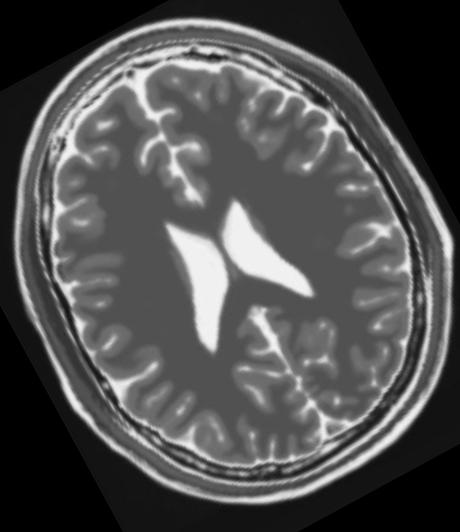
\includegraphics[scale=0.3]{J3.jpg}
\caption{Rotated Image J3}
\end{figure}

\newpage
\subsection*{(b)}

The MATLAB code for this question is as follows:
\begin{lstlisting}[frame=single,numbers=left,style=Matlab-Pyglike,breaklines=true,postbreak=\mbox{\textcolor{red}{$\hookrightarrow$}\space}]
    angles = -45:1:45;

    ncc = zeros(size(angles));
    je = ncc;
    qmi = ncc;
    
    for i = 1:length(angles)
        J4 = imrotate(J3, angles(i), 'bilinear', 'crop');
        J4(isnan(J4)) = 0;
        
        normJ4 = (J4 - mean(J4(:))) / std(J4(:));
        normJ1 = (J1 - mean(J1(:))) / std(J1(:));
        
        ncc(i) = sum(normJ1(:) .* normJ4(:)) / numel(J1);
        
        jointHist = histcounts2(normJ1(:), normJ4(:), 7); % 256^(1/3) bins approximately
        jointProb = jointHist / sum(jointHist(:));
        je(i) = -sum(jointProb(jointProb > 0) .* log2(jointProb(jointProb > 0)));
        
        P1 = sum(jointProb, 1);
        P2 = sum(jointProb, 2);
        P1P2 = zeros(length(P1));
        for j = 1:length(P1)
            for k = 1:length(P2)
                P1P2(j, k) = P1(j) * P2(k);
            end
        end
        qmi(i) = sum(sum((jointHist - P1P2).^2));
    end
\end{lstlisting}

\newpage
\subsection*{(c)}

The plots for the three dependence measures are as follows:
\begin{figure}[H]
\centering
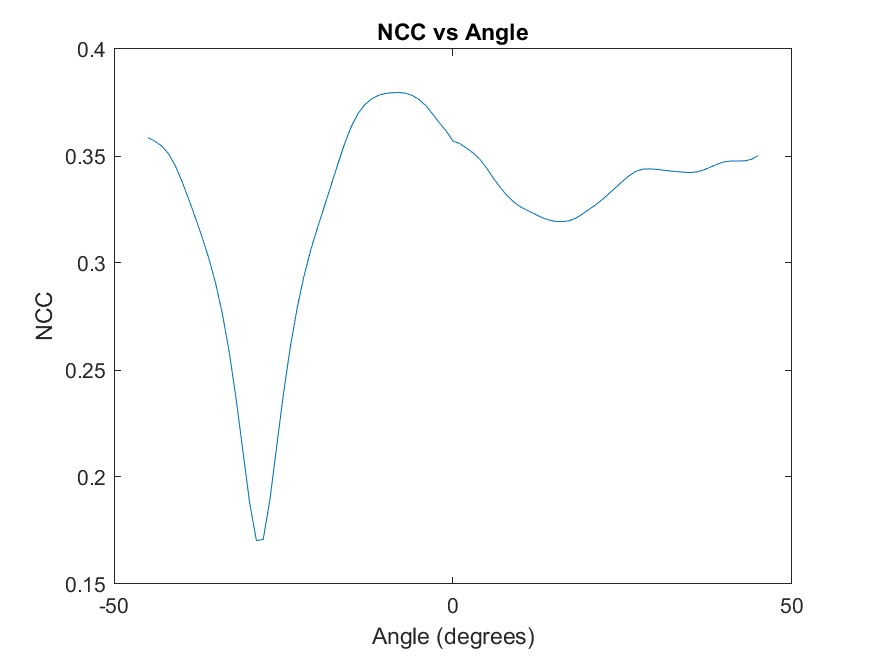
\includegraphics[scale=0.3]{NCC_vs_Angle.jpg}
\caption{Normalized Cross Correlation}
\end{figure}

\begin{figure}[H]
\centering
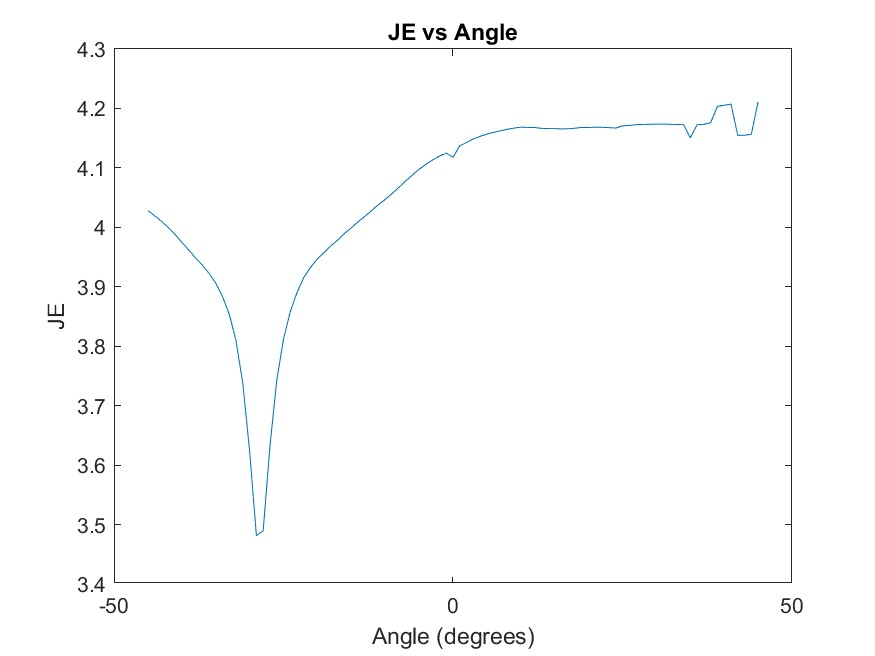
\includegraphics[scale=0.3]{JE_vs_Angle.jpg}
\caption{Joint Entropy}
\end{figure}

\begin{figure}[H]
\centering
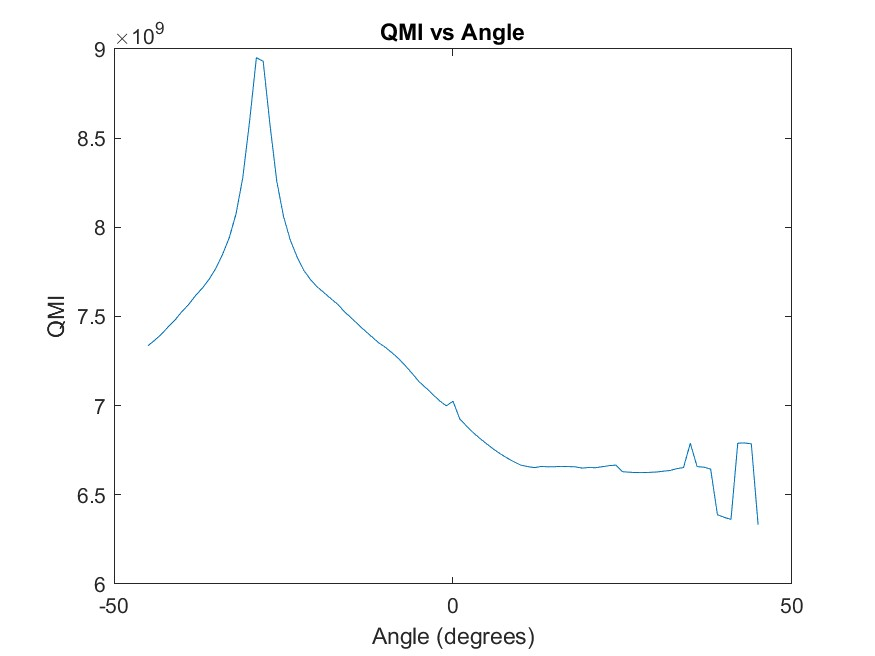
\includegraphics[scale=0.3]{QMI_vs_Angle.jpg}
\caption{Quadratic Mutual Information}
\end{figure}

\subsection*{(d)}

The MATLAB code for this question is as follows:
\begin{lstlisting}[frame=single,numbers=left,style=Matlab-Pyglike,breaklines=true,postbreak=\mbox{\textcolor{red}{$\hookrightarrow$}\space}]
    [~, nccIndex] = min(ncc);
    [~, jeIndex] = min(je);
    [~, qmiIndex] = max(qmi);
    
    fprintf('Best NCC angle: %.2f degrees (NCC value: %.4f)\n', angles(nccIndex), ncc(nccIndex));
    fprintf('Best JE angle: %.2f degrees (JE value: %.4f)\n', angles(jeIndex), je(jeIndex));
    fprintf('Best QMI angle: %.2f degrees (QMI value: %.4f)\n', angles(qmiIndex), qmi(qmiIndex));    
\end{lstlisting}

From the plots, the best angle for the three dependence measures comes out to be \textbf{$29^{\circ}$ counter-clockwise}. We observe that at this angle, the NCC value is minimized, the JE value is minimized and the QMI value is maximized.
Thus all the three dependence measures agree on the best angle of rotation.

\vspace{5pt}
\texttt{Terminal Out:\\Best NCC angle: -29.00 degrees (NCC value: 0.1703)\\
Best JE angle: -29.00 degrees (JE value: 3.4815)\\
Best QMI angle: -29.00 degrees (QMI value: 8951113300.4131)}

\newpage
\subsection*{(e)}

The optimal angle of rotation is $29^{\circ}$ counter-clockwise. The MATLAB code for this question is as follows:
\begin{lstlisting}[frame=single,numbers=left,style=Matlab-Pyglike,breaklines=true,postbreak=\mbox{\textcolor{red}{$\hookrightarrow$}\space}]
    optimJ4 = imrotate(J3, angles(jeIndex), 'bilinear', 'crop');
    optimJ4(isnan(optimJ4)) = 0;
    
    bins = 37; % 256/7 approximately
    
    histJ1 = histcounts(J1(:), bins);
    histJ4 = histcounts(optimJ4(:), bins);
    
    jointHist = zeros(bins);
    
    for i = 1:size(J1, 1)
        for j = 1:size(optimJ4, 2)
            intensity_bin1 = floor(J1(i, j) * (bins - 1)) + 1;
            intensity_bin2 = floor(optimJ4(i, j) * (bins - 1)) + 1;
            jointHist(intensity_bin1, intensity_bin2) = jointHist(intensity_bin1, intensity_bin2) + 1;
        end
    end
    
    % Normalize the joint histogram to create a joint probability distribution
    jointProb = jointProb / sum(jointHist(:));
    
    % Plot the joint histogram
    figure; imagesc(jointProb);
    colormap jet;
    colorbar;
    xlabel('Intensity in J4 (Rotated)');
    ylabel('Intensity in J1');
    title('Joint Histogram between J1 and J4 (Optimal JE)');
    axis xy;
     
    % Save the plot as an image
    saveas(gcf, 'JointHist_Optimal_JE.jpg');
\end{lstlisting}

The joint histogram between the original image J1 and the optimally rotated image J4 is as follows:
\begin{figure}[H]
\centering
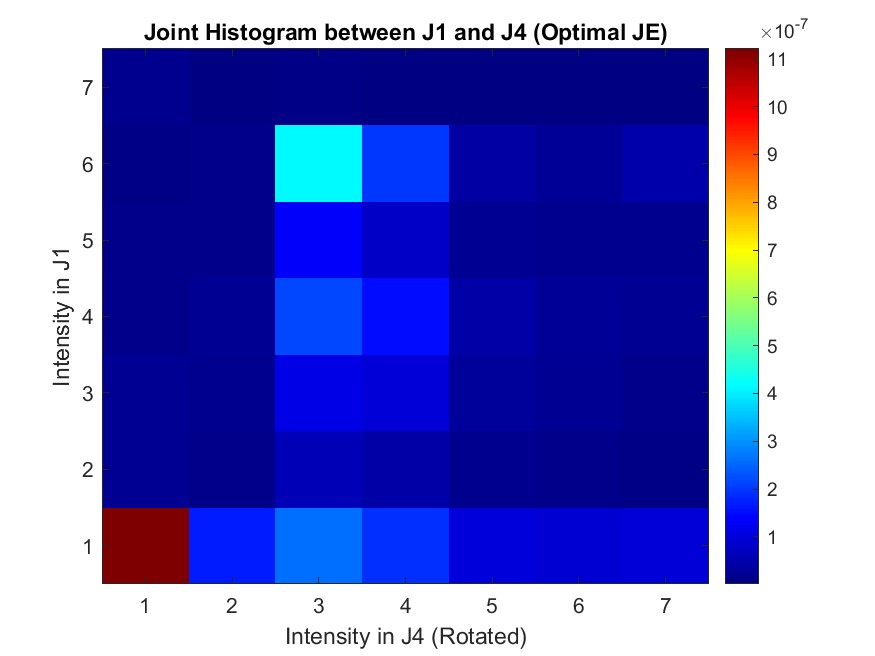
\includegraphics[scale=0.3]{JointHist_Optimal_JE.jpg}
\caption{Joint Histogram between J1 and J4 (Optimal JE)}
\end{figure}

\subsection*{(f)}
Quadratic Mutual Information (QMI) measures the statistical relationship between the two random variables, such as pixel intensities in images. It compares the actual joint distribution of these variables to the expected distribution if they were independent.
\vspace{5pt}

If the variables are independent, their joint distribution will be similar to the product of their individual distributions, resulting in a low QMI value. But if the variables are dependent, the joint distribution differs leading to a much higher QMI value.
\vspace{5pt}

Hence, QMI helps identify and quantify the dependence between two variables, capturing details that might not be evident with other measures.

\end{document}